This exercise has been completed in the attached \textit{K\_Means.ipynb} Jupyter Notebook. The most relevant bits of source code can be seen here as well, though all comments are left out. The final version is also different, as the function has to accommodate larger images. The function remains unchanged for this image though:
\begin{verbatim}
def makeNewImg(image, n_clusters, max_iter, seed):
    imgx   = image.shape[0]
    imgy   = image.shape[1]
    imgRGB = image.shape[2]
    model  = KMeans(n_clusters, max_iter, seed)
    image  = image.reshape((imgx*imgy),imgRGB)
    model.fit(image)
    
    retval = np.zeros(((imgx*imgy),imgRGB))

    for i in range(n_clusters):
        for j in range(imgRGB):
            model.cluster_means[i,j] = 
                model.cluster_means[i,j]/255
            
    for i in range(retval.shape[0]):
        retval[i] = 
            model.cluster_means[model.cluster_assignments[i]]
        
    retval = retval.reshape((imgx,imgy,imgRGB))
    return retval, model.cluster_means
\end{verbatim}
The 5 cluster means, calculated using the Jupyter Notebook, look as follows. It should be noted that they are all RGB values, but Python wants RGB values in one of two forms; floats between $0$ and $1$, or integers between $0$ and $255$. Here they are floats between $0$ and $1$:
$$
\begin{matrix}
[0.41773344, 0.71691352, 0.84028094] \\[3pt]
[0.13106363, 0.12181295, 0.11628755] \\[3pt]
[0.47558986, 0.42848816, 0.35511877] \\[3pt]
[0.76865056, 0.87663444, 0.90978927] \\[3pt]
[0.75330927, 0.69978601, 0.48412478] \\[3pt]
\end{matrix}
$$
The assigned cluster for each pixel has been calculated, and the new image has been plotted:\\
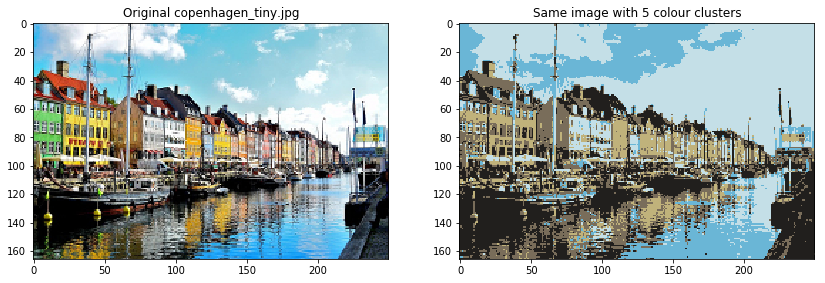
\includegraphics[width=\linewidth]{3b1.png}\\